% !TEX encoding = UTF-8 Unicode

\section{Organização da memória}

O ambiente de execução da MVN fornece aos programadores um tamanho limitado de memória para ser usado no geral, a ser compartilhado entre o código e as variáveis do programa. O montador aloca a memória com base nos endereços relativos especificados no código do programa. Do total, a parte inicial da memória é reservada para guardar as instruções que serão executadas pelo programa. A parte final da memória deve ser usada especialmente para o uso do registro de ativação.

De maneira mais objetiva, reserva-se uma parte do código para a área de dados, uma parte para a função principal e as subrotinas e uma parte dedicada a pilhas de variáveis e endereços que viabilizam a chamada de subrotinas.

\section{Registro de ativação}

As funções em programas têm variáveis locais, que devem ser criadas na chamada da função e sobrevivem até que a função retorne. Elas também possuem recursão, onde cada instância da função tem seus próprios parâmetros e locais. As chamadas de funções se comportam de maneira LIFO, portanto podemos usar uma pilha como estrutura.

As operações push e pop dessa pilha não podem ser feitas individualmente para cada variável. Desa forma, manipula-se conjuntos de variáveis, e precisamos ter acesso a todas elas. Com isso, definimos dois conceitos:

\begin{itemize}
	\item \emph{Stack Pointer} (SP):
	\begin{itemize}
		\item Todas as posições além do SP são lixo;
		\item Todas as anteriores estão alocadas.
	\end{itemize}
	
	\item \emph{Activation Record} ou \emph{Stack Frame}
	\begin{itemize}
		\item área na pilha reservada para os dados de uma função (parâmetros, locais, endereço de retorno, etc).
	\end{itemize}
\end{itemize}

\begin{figure}[ht]
	\centering
	\caption{Esquema do Registro de Ativação}
	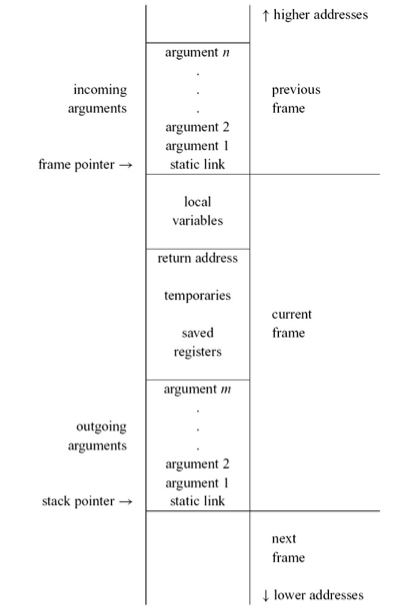
\includegraphics[width=0.5\textwidth]{images/registros-ativacao.png}
	\label{fig:registros-ativacao}
\end{figure}

A figura~\ref{fig:registros-ativacao} ilustra a organização da pilha. O uso do registro de ativação permite entre outras coisas a chamada recursiva de funções, uma vez isso não é possível de forma nativa no ambiente da MVN. No caso da MVN, a pilha cresce para baixo e as subrotinas são executadas utilizando as seguintes instruções:

\begin{itemize}
	\item Desvio para subprograma - mnemônico SC (0xA): armazena o endereço de instrução seguinte (atual + 1) na posição de memória apontada pelo operando. Em seguida, desvia a execução para o endereço indicado pelo operando e acrescido de uma unidade.
	
	\item Retorno de subprograma - mnemônico RS (0xB): desvia a execução para o endereço indicado pelo valor guardado na posição de memória do operando.
\end{itemize}

Foi criado por nós uma biblioteca em assembly para implementar funções auxiliares de entrada e saída de dados, além da funcionalidade de empilhar, desempilhar e ter acesso a informações contidas na pilha discutida anteriormente. Essas funções são explicadas na próxima seção.
